
\documentclass[12pt]{standalone}
\usepackage{amssymb,latexsym, amsmath,graphics}
\usepackage{amsthm}
\usepackage{setspace}

\doublespacing

\usepackage{pgf}
\usepackage{tikz}
\usetikzlibrary{arrows,automata}
\usetikzlibrary{positioning}

\begin{document}
\pagestyle{empty}
 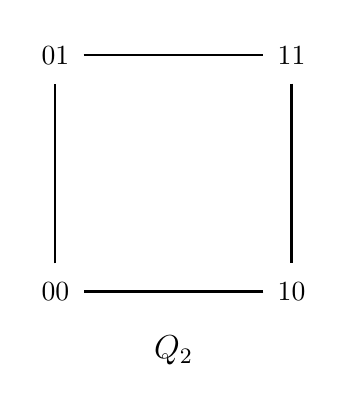
\begin{tikzpicture} [scale=3]
	 \tikzstyle{vertex}=[circle,minimum size=20pt,inner sep=0pt]
	 \tikzstyle{edge} = [draw,thick,-,black]
	 \node[vertex] (v0) at (0,0) {$00$};
	 \node[vertex] (v1) at (0,1) {$01$};
	 \node[vertex] (v2) at (1,0) {$10$};
	 \node[vertex] (v3) at (1,1) {$11$};

	 \draw[edge] (v0) -- (v1) -- (v3) -- (v2) -- (v0);
	 
	 \node[] at (.5,-.25) {\large $Q_2$};

 \end{tikzpicture}
\end{document}